\documentclass{scrartcl}
\usepackage[utf8]{inputenc}
\usepackage[T1]{fontenc}
\usepackage{graphicx}
\usepackage{wrapfig,lipsum}
\usepackage{hyperref}
\usepackage{float}
\usepackage{enumitem}
\usepackage{fmtcount}
\usepackage{eurosym}
\usepackage{amstext} % for \text
\DeclareRobustCommand{\officialeuro}{%
  \ifmmode\expandafter\text\fi
  {\fontencoding{U}\fontfamily{eurosym}\selectfont e}}
\usepackage[dvipsnames]{xcolor} %for alloy package
\usepackage{listings}
\usepackage{algorithm}
\usepackage[noend]{algpseudocode}
\usepackage{pdflscape}


\title{Software Engineering 2: "PowerEnJoy"\newline\newline
Design Document}
\subtitle{Version 1.0}
\author{Piccirillo Luca - 790380\\
Zampogna Gian Luca - 863097\\
Zini Edoardo - 875275}
\date{December 11\textsuperscript{th}, 2016}

\hypersetup{
    colorlinks,
    citecolor=black,
    filecolor=black,
    linkcolor=black,
    urlcolor=black
}

\begin{document}
\pagenumbering{gobble}
\begin{figure} [h!]
    \centering
    
\includegraphics[scale=0.6]{{Figures/LogoPolimi.png}}
    \label{fig:LogoPolimi}
    \maketitle
\end{figure}
\newpage
\pagenumbering{roman}
\tableofcontents
\newpage
\pagenumbering{arabic}

\section{Introduction}
\subsection{Purpose}


\subsection{Scope}


\subsection{Definitions, Acronyms, Abbreviations}
\subsubsection{Acronyms, Abbreviations}
\begin{itemize}
    \item PEJ = PowerEnJoy
    \item SBL = Service Back-end Logic: software logic of the service the user do not directly interact with.
\end{itemize}
\subsubsection{Definitions}
\begin{itemize}
\item \textbf{Car:} every vehicle, which respects the requirements, that the system allows the users to use.
    \item \textbf{Special Parking Area:} pre-defined areas (i.e. streets) where a user is allowed to park and where the batteries of the Cars can be plugged into the power grid.
    \item \textbf{Total Base Fare:} amount of money that the user pays for the ride duration only. It does not include any discount or penalty for any other specific condition.
    \item \textbf{Total Ride Fare:} amount of money that the user pays. It includes any discount or penalty for any other specific condition satisfied during the ride.
\end{itemize}

\subsection{Reference Document}
\begin{itemize}
    \item Project?s Assignment document: AA 2016-2017 Software Engineering 2 - Project goal, schedule, and rules.
    \item IEEE Std 830-1998, IEEE Recommended Practice for Software Requirements Spec- ifications.
    \item Software Engineering 2: "PowerEnJoy" Requirements Analysis and Specification Document.
    \item UX diagram PDF from the course "Sistemi Informativi" of Politecnico of Milan.
\end{itemize}

\subsection{Document Structure}
This document is split in 6 parts:
\begin{itemize}
    \item \textbf{Architectural Design:} contains the different architectural views of the system.
    \item \textbf{Algorithm Design:} contains the pseudo-codes of the most relevant algorithmic parts of the system.
    \item \textbf{User Interface Design:} contains an overview of how the user interface on the system will look like.
    \item \textbf{Requirements Traceability:} shows the correlation among the requirements defined in the RASD and the design elements contained in this document.
    \item \textbf{Effort Spent:} contains the amount of time each member spent on the document, split between time spent working together and time spent on his own.
    \item \textbf{References:} contains all the references required by this document.
\end{itemize}
\newpage
\section{Architectural Design}

\subsection{High level components and interactions}
The following block diagram describes the overall solution design by giving an high-level perspective of all main application roles. In particular, it makes easy to understand the partition of software service components across the solution realm and their interaction mechanisms through internal subsystems interfaces.

\begin{figure} [h!]
\centering
\includegraphics[scale=0.66]{{Figures/Architecture.png}}
\label{fig:Architecture}
\end{figure}

% \begin{wrapfigure}{r}{5.5cm}
% \caption{A wrapped figure going nicely inside the  text.}\label{wrap-fig:1}
% \includegraphics[width=5.5cm]{Figures/Architecture.png}
% \end{wrapfigure} 
%------------------------------------------
% {\lipsum[2-3]
% \par
% Figure~\ref{wrap-fig:1} is a wrapped figure.}


\begin{itemize}
\item{\textbf{Client side applications}}\newline
Represent the pool of user interactive applications made of both mobile applications running on user owned devices and onboard ride assistants running on the onboard infotainment devices of PowerEnJoy Cars.
\item{\textbf{Vehicle management platforms}}\newline
Represent the pool of embedded controllers devoted to remotely interfacing the vehicle hardware.

\item{\textbf{Front-end service roles}}
\begin{itemize}
\item{\textbf{Client Worker}}\newline
A single Client Worker node acts as a proxy between any remote interactive client and back-end components. In other words, it exposes all interfaces needed by any application the end user directly interacts with to allow decoupling from core service feature components, avoiding any client technology-dependent issue to be addressed by back-end design decisions. It is able to validate an existing authentication token avoiding redundant messaging to the back-end. It also provides access to static/cached resources and it's designed to be fully stateless, allowing automatic/on-demand scale-up of nodes instances to distribute workload across, dramatically increasing reliability and performance. A Client Worker node can return execution results to remote clients both in synchronous (request/response) or asynchronous mode (event/notification).
\item{\textbf{Vehicle Worker}}\newline
A single Vehicle Worker node acts as a proxy between any remote supported vehicle platform and back-end components. In other words, it exposes all interfaces needed by any supported vehicle to allow decoupling from core service feature components, avoiding any platform-dependent issue to be addressed by back-end design decisions. It's designed to manage and keep track of an huge number of status/telemetry updates. Inside a Vehicle Worker node, updates from multiple different vehicles are stored until expiration and timestamped. When an event is triggered by a new vehicle the node registers itself to the back-end as the handler of that vehicle. This way we are still allowing automatic/on-demand scale-up of nodes instances to distribute workload across, dramatically increasing reliability and performance. A Vehicle Worker node works only in asynchronous mode (event/notification) w.r.t. the remote vehicle.
\item{\textbf{Elastic load balancing request router}}\newline
Available from any common cloud provider. Provides automatic scale-up/-down of nodes instances based on their resources utilization and redirects request messages to nodes guaranteeing a fair workload distribution across them.
\item{\textbf{Elastic load balancing event hub}}\newline
Available from any common cloud provider. Provides automatic scale-up/-down of nodes instances based on their resources utilization and manages to forward an huge number of event messages to nodes guaranteeing a fair workload distribution across them.
\item{\textbf{Elastic async push messages dispatcher}}\newline
Available from any common cloud provider. Provides efficient queuing of large number of messages to dispatch to multiple groups of targets. It also takes care of creating and keeping up network notification channels.
\end{itemize}

\item{\textbf{Back-end service roles}}
\begin{itemize}
\item{\textbf{Service Business Logic Worker}}\newline
Each SBL Worker node provides all PowerEnJoy core service features. They actually runs the whole service logic decoupled from any presentation layers and communication protocols to front-end devices. Each SBL Worker is fully stateless and supports simultaneous multiple worker's instances with obvious redundancy and performance advantages. For better performances a single node is restricted by design to serve only a specific service zone. An SBL Worker also provides some data access optimization (i.e. caching, mirroring) to inner components and can be instantiated both automatically by scaling managers or manually if needed. For example, if interface compatibility is preserved, it will be possible to manually instantiate an SBL Worker running a different software version, allowing seamless on-field testing, debugging and upgrade experience.
\item{\textbf{Elastic load balancing service bus}}\newline
Available from any major cloud provider. Allows efficient interconnection of components between back-end and front-end roles. It can be configured to act as an automatic scaling manager if the cloud provider offers that option.
\item{\textbf{User Account Data}}\newline
Stores all account related data such as user credentials, personal identity, driving license, credit card details and payments history. Accounts are unique and shared across all PowerEnJoy covered zones.
\item{\textbf{Configuration Data}}\newline
Stores all service global parameters that system administrators can modify according to their needing, like those related to discounts and penalties policies, service fares, booking timeouts and so on.
\item{\textbf{Single Zone Data}}\newline
Stores all data related to a single zone covered by the PowerEnJoy service such as vehicles, Safe and Special Parking Areas, active bookings and any parameter override that should only be applied to that zone.
\item{\textbf{Management API}}\newline
Provides administrative and monitoring low-level access to core components, designed to be easily interfaced with any business management platform (ERP, CRM, enterprise portals, etc.). It's existence has been taken into account only to adapt current solution design for future software evolution. No further design or development effort will be spent on this component unless requirements renegotiation. As of this document revision, the described solution is fully functional and serviceable without this component by direct manipulation of data.
\end{itemize}
\end{itemize}

\subsection{Component view}
This section contains the component view and the descriptions of each component. Their interfaces are described in the section component interfaces (2.5).
\subsubsection{Service Business Logic}
\begin{figure} [h!]
\centering
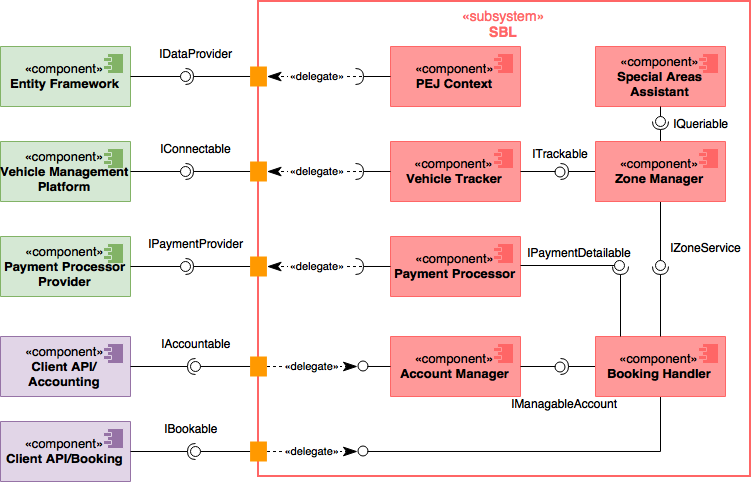
\includegraphics[scale=0.5]{{Figures/Component_Diagram/SBL.png}}
\label{fig:SBL}
\end{figure}
The Service Business Logic subsystem is composed of:
\begin{itemize}
    \item\textbf{PEJ Context}\newline
    It is the component through which all the others can access data entities containing all the information and details about zone, vehicles, accounts, configurations, bookings, rides and payments.
    \item\textbf{Zone Manager}\newline
    It is the component that connects Booking Handler to related Vehicle Tracker and Special Parking Areas of inherent zone applying any zone-specific configurations.
    \item\textbf{Special Areas Assistant}\newline
    It is the component that provides the set of functions needed to get lists of Special Parking Areas satisfying specific requirements.
    \item\textbf{Vehicle Tracker}\newline
    It is the component that asynchronously interacts with the Vehicle Management Platform collecting data required by other components.
    \item\textbf{Booking Handler}\newline
    It is the component that manages the bookings and their related rides. It provides the functions for creating a new booking, having it progress to a ride and ending it creating a pending payment record of appropriate amount.
    \item\textbf{Payment Processor}\newline
    It is the component in charge of managing pending payments issuing requests to Payment Processor Provider.
    \item\textbf{Account Manager}\newline
    It is the component in charge of managing user data when he creates a new account, signs in, asks for his personal profile page or wants to modify personal details.
\end{itemize}
and it interacts with:
\begin{itemize}
    \item\textbf{Entity Framework}\newline
    It is the set of external sub-components that is in charge of binding data entity models to corresponding datasource schema.
    \item\textbf{Live Vehicle API}\newline
    It is the component that connects to a vehicle management platforms in order to get live data including positions, battery level, engine ignited, and all the other data provided by the vehicle sensors.
    \item\textbf{Payment Processor Provider}\newline
    It is the third party system PowerEnJoy relies on in order to bill the customer's credit cards.
    \item\textbf{Client API/Accounting}\newline
    It is the middleware between SBL and client-side apps the user interact with. It exposes only the set of interfaces required to register, sign in or modify the personal user data.
    \item\textbf{Client API/Booking}\newline
    It is the middleware between SBL and client-side apps the user interact with. It exposes the set of interfaces required to create or cancel a reservation, and manage the whole ride including access to the map of available vehicles, the position of the reserved Car or to get lists of Special Parking Areas.
    \item\textbf{Mail Server}\newline
    It is the component in charge of sending to the specified user the mail containing payment result and details of the ride.
\end{itemize}
%Add \newpage here if necessary
%\newpage

\subsubsection{User Device Mobile App}
\begin{figure} [h!]
\centering
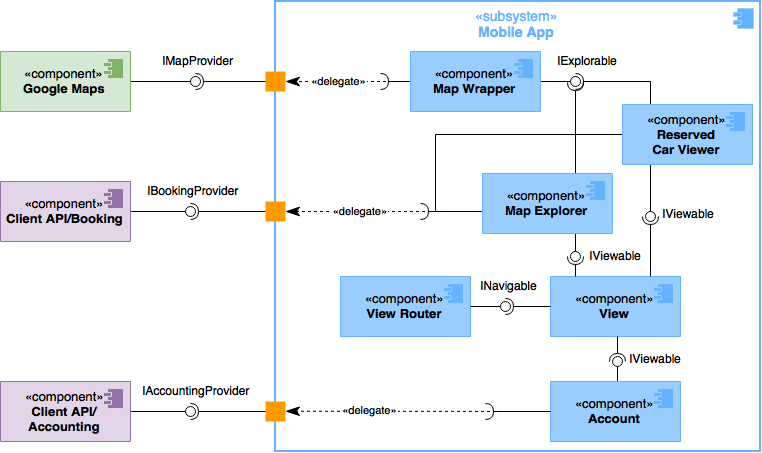
\includegraphics[scale=0.5]{{Figures/Component_Diagram/MobileApp.png}}
\label{fig:MobileApp}
\end{figure}
The User Device Mobile App is composed of:
\begin{itemize}
    \item\textbf{View}\newline
    It is a set of sub-components representing something the user can see and interact with; each sub-component renders the view relying on the view models provided by other components and translates user inputs to well-formed and sanitized requests sent through other components.
    For this application this set includes sub-components related to map, sign-in and sign-up forms, account and reservation management.
    \item\textbf{View Router}\newline
    It is the component that implements and keep tracks of navigation paths across various views, providing for a given view model the right view component to be navigated that is able to present it to the user. It also implements backward navigation feature.
    \item\textbf{Map Wrapper}\newline
    It is the component that wrap the outsourced map images into an user control that makes them scrollable and zoomable, with the ability to overlay custom objects in defined position. It allows the application not to be coupled to a specific third-party maps provider.
    \item\textbf{Map Explorer}\newline
    It is the component that takes the map provided by the Map Wrapper and takes care of showing the position of all available Cars on that map. These positions are obtained via Client API/Booking call.
    \item\textbf{Reserved Car Viewer}\newline
    It is the component that takes the map provided by the Map Wrapper and adds the position of the reserved Car. This position is stored within the app or it is requested via Client API/Booking call if necessary. It allows the user to request a booking cancellation or the unlock of its associated Car.
    \item\textbf{Account}\newline
    It is the component in charge of all the account-related functions. After the sign in, it provides the view with the user avatar, so that it can be used as access to the user personal data page which is also managed by this component.
\end{itemize}
and it interacts with:
\begin{itemize}
    \item\textbf{Google Maps}\newline
    It is the third party map provider whose maps are used in the user device mobile app.
    \item\textbf{Client API/Accounting}\newline
    \textit{See above.}
    \item\textbf{Client API/Booking}\newline
    \textit{See above.}
\end{itemize}
%Add \newpage here if necessary
%\newpage

\subsubsection{Onboard Ride Assistant App}
\begin{figure} [h!]
\centering
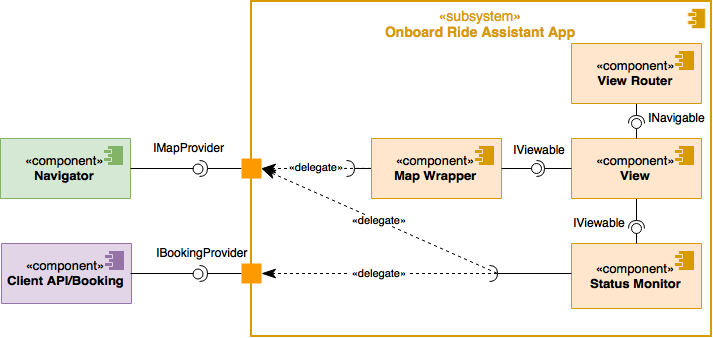
\includegraphics[scale=0.5]{{Figures/Component_Diagram/CarApp.png}}
\label{fig:CarApp}
\end{figure}
The Onboard Ride Assistant App is composed of:
\begin{itemize}
    \item\textbf{View}\newline
    It is a set of sub-components representing something the user can see and interact with; each sub-component renders the view relying on the view models provided by other components and translates user inputs to well-formed and sanitized requests sent through other components.
    For this application this set includes sub-components related to navigator, search input field, options and ride details.
    \item\textbf{View Router}\newline
    It is the component that implements and keep tracks of navigation paths across various views, providing for a given view model the right view component to be navigated that is able to present it to the user. It also implements backward navigation feature.
    \item\textbf{Map Wrapper}\newline
    It is the component that wraps the maps provided by the Navigator and makes it scrollable and zoomable, with the ability to overlay custom objects in defined position. It allows the application not to be coupled to a specific third-party navigation product.
    \item\textbf{Status Monitor}\newline
    It is the component that updates the ride details and the options available to the user: money saving alternative destination and Special Parking Areas listing.
\end{itemize}
and it interacts with:
\begin{itemize}
    \item\textbf{Navigator}\newline
    It is the third-party navigation software which provides navigation directions to the user, and translate the inserted addresses into precise coordinates. It also provides maps images to other components.
    \item\textbf{Client API/Booking}\newline
    \textit{See above.}
\end{itemize}
%Add \newpage here if necessary
\newpage

\subsection{Deployment view}
\begin{figure} [h!]
\centering
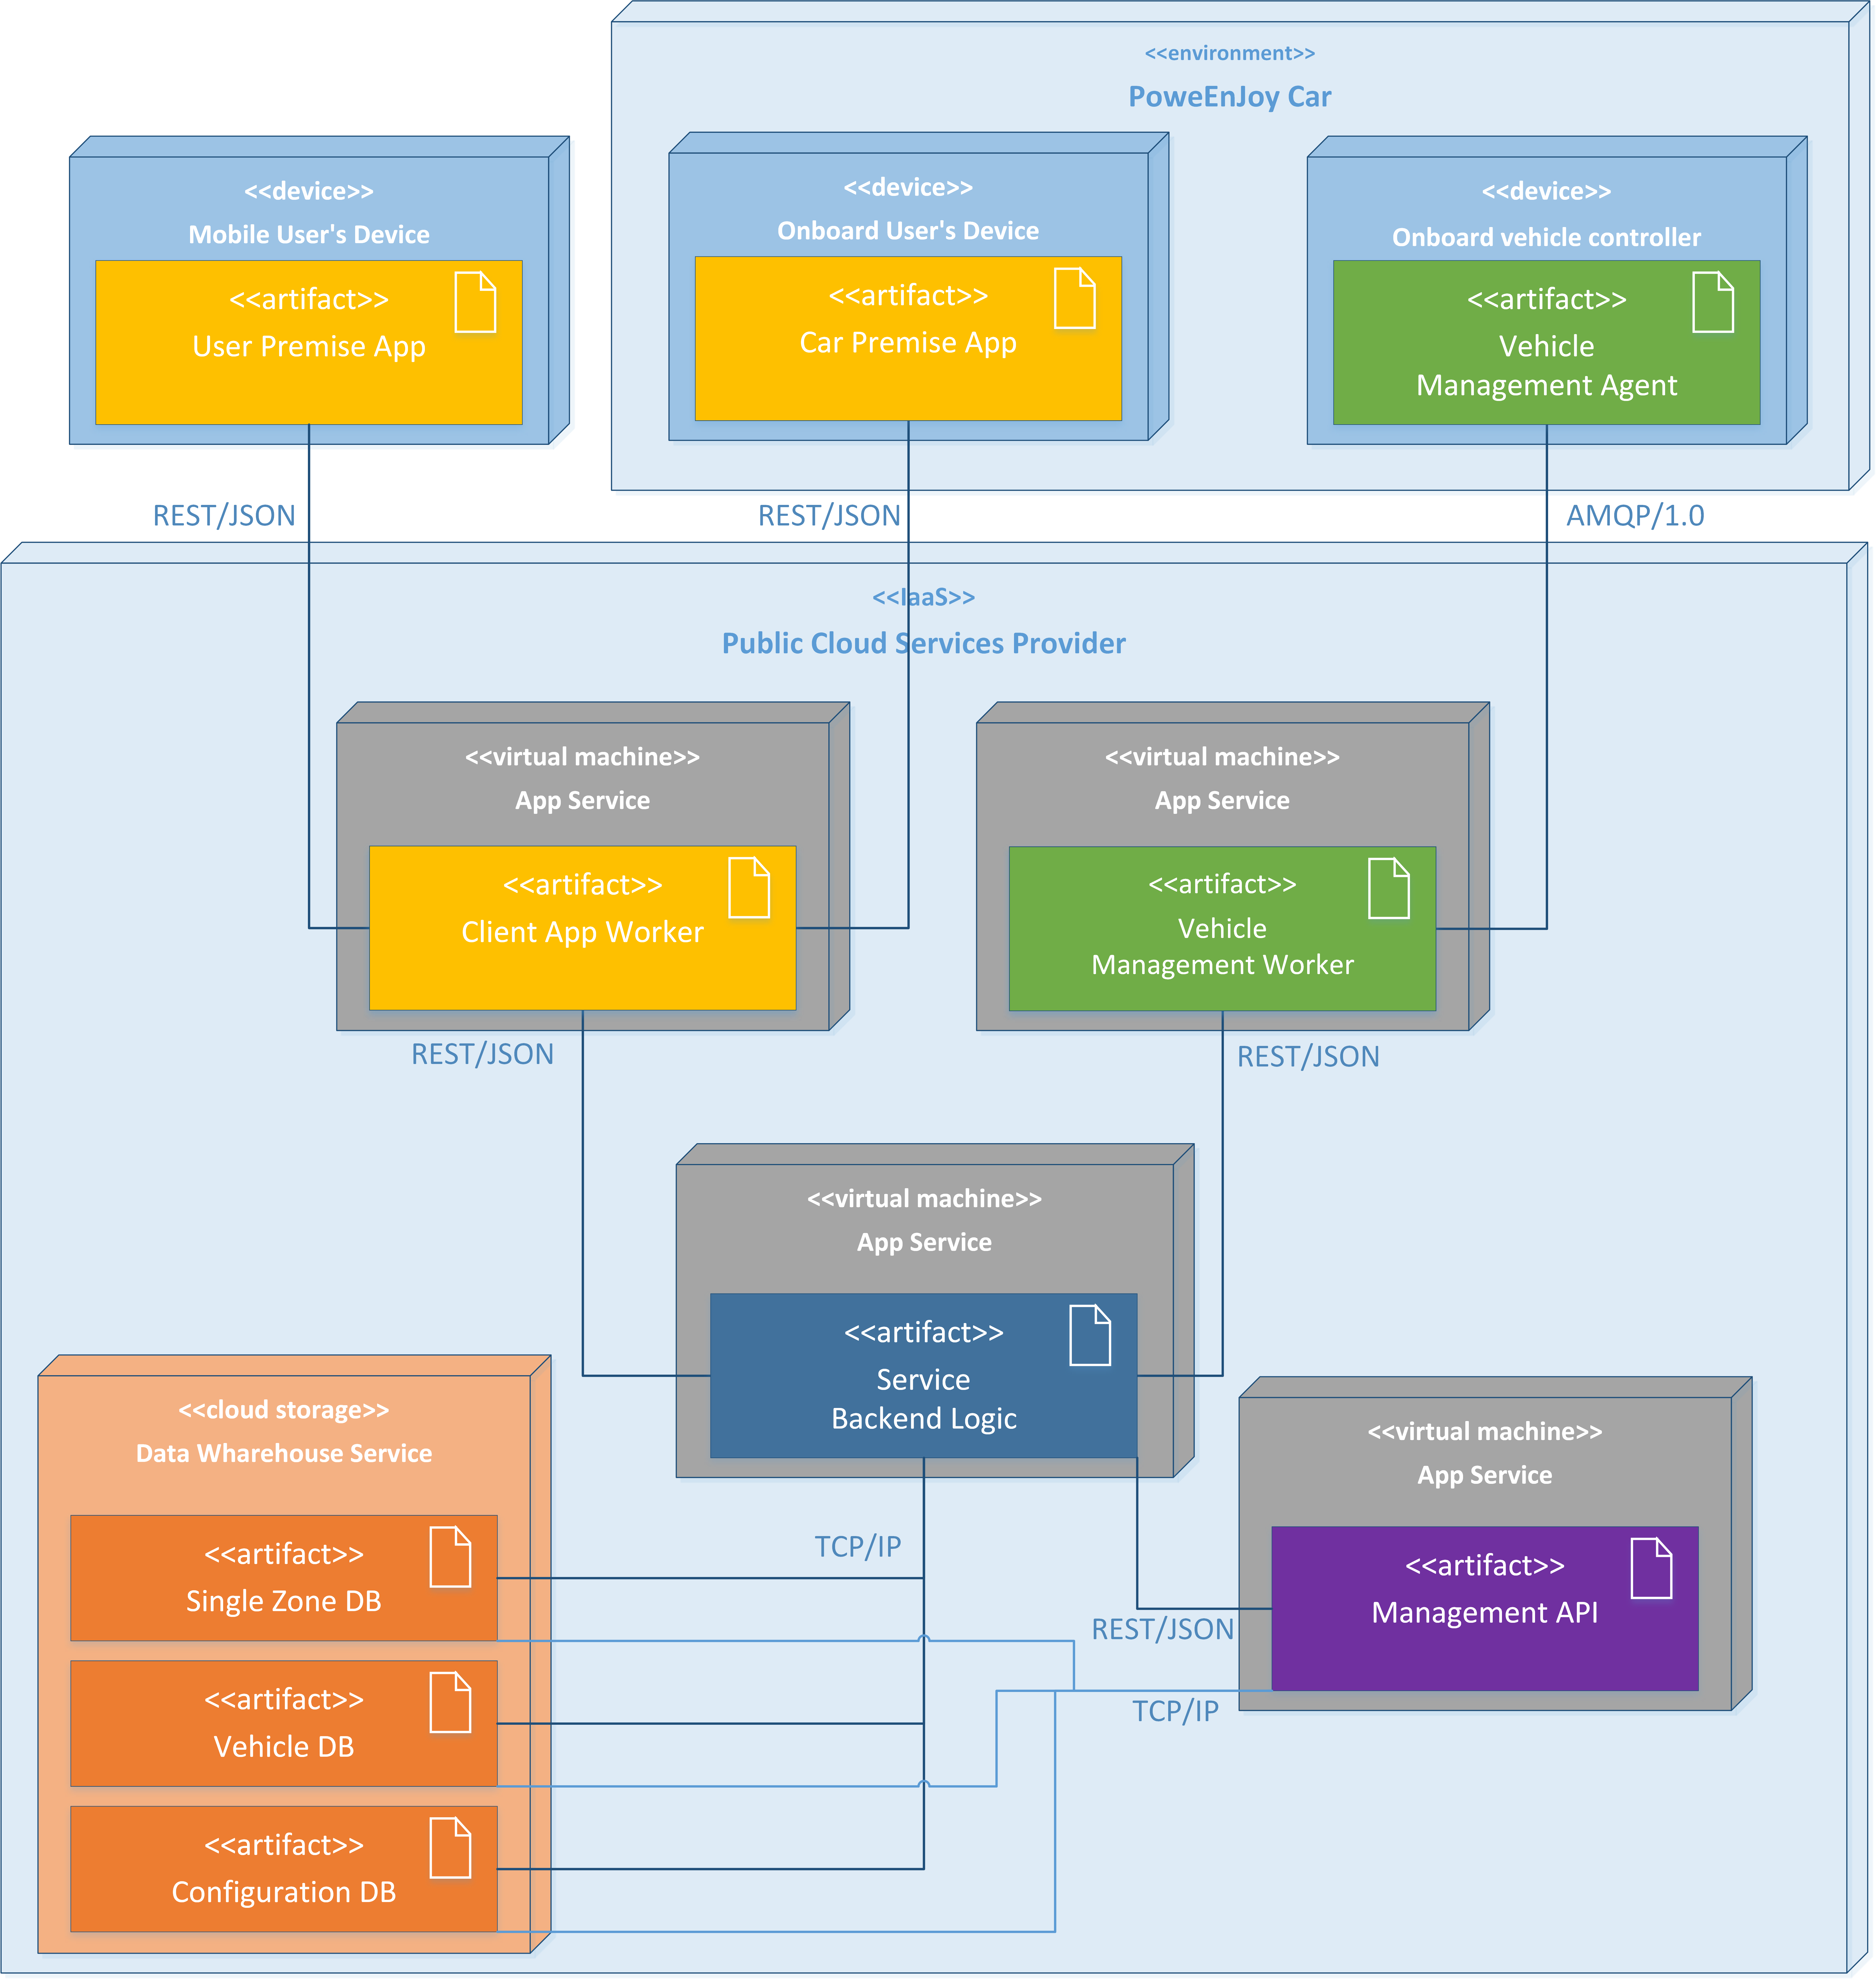
\includegraphics[scale=0.51]{{Figures/Deployment.png}}
\label{fig:Deployment}
\end{figure}
\begin{itemize}
    \item\textbf{Mobile User's device}\newline
    It's the mobile device owned by a generic user. He can download and install the PowerEnJoy application via platform specific app. Any major mobile systems are supported.
    \item\textbf{PowerEnJoy Car}
    \begin{itemize}
        \item\textbf{Onboard User's Device}\newline
        It's the device which every Car is equipped with, it executes a preloaded interactive application, and includes the third-party navigator software along with offline map data. This device also shares GPS sensor data and Internet connectivity with any other onboard device.
        \item\textbf{Onboard Vehicle Controller}\newline
        It's an embedded device which every Car is equipped with, it's connected to Car hardware interface and sensor pool.
    \end{itemize}
    \item\textbf{Public Cloud Service Provider}
    \begin{itemize}
        \item\textbf{App Service}\newline
        It's an IaaS virtual machine already configured to run web-based services. It can be replicated into new instances by scaling managers. The app service setup is stored in virtual storage and every app service instance has access to a virtual copy of that setup. The deployment is managed by continuous integration services or other specific tools by the cloud provider. Most software components of this solution runs on such kind of compute units.
        \item\textbf{Data Wharehouse Service}\newline
        It's a virtual relational data storage, running on a DBaaS environment. Every database for PowerEnJoy take place in this cluster but each database can also be configured to be phisically located in preferred country or region in case of regulatory constraints.
    \end{itemize}
    \item\textbf{Communication protocols}\newline
    For a comprehensive description of deployed communication protocols refer to section §\ref{com_patterns}.
\end{itemize}
%Add \newpage here if necessary

\subsection{Runtime view}

This section contains some Sequence Diagrams of the application.\\
In particular it shows what happens whenever:
\begin{itemize}
\item User send a request for unlock the Car;
	\newline in this diagram the SBL communicates with Car using asynchronous messages: SBL send messages to Live Vehicle API that route them to the car and answer once has the information required.
\item User set ride destination and drive towards it; the third diagram extends the second one and shows the Special Parking Area List and the Money Saving option features.
\newline in this diagram SBL communicates with Car through synchronous messages because we implies Live Vehicle API usage.
\end{itemize}

\newpage

\begin{landscape}
\begin{figure} [h!]
\centering
\includegraphics[scale=0.6]{{Figures/Sequence_Diagram/CarUnlock.png}}
\label{fig:UML Sequence Diagram: Car unlocking}
\caption{Car Unlocking}
\end{figure}
\end{landscape}

\newpage
\begin{landscape}
\begin{figure} [h!]
\centering
\includegraphics[scale=0.6]{{Figures/Sequence_Diagram/Ride.png}}
\label{fig:UML Sequence Diagram: Ride}
\caption{User's ride}
\end{figure}
\end{landscape}

\newpage

\begin{figure} [h!]
\centering
%scale=0.46
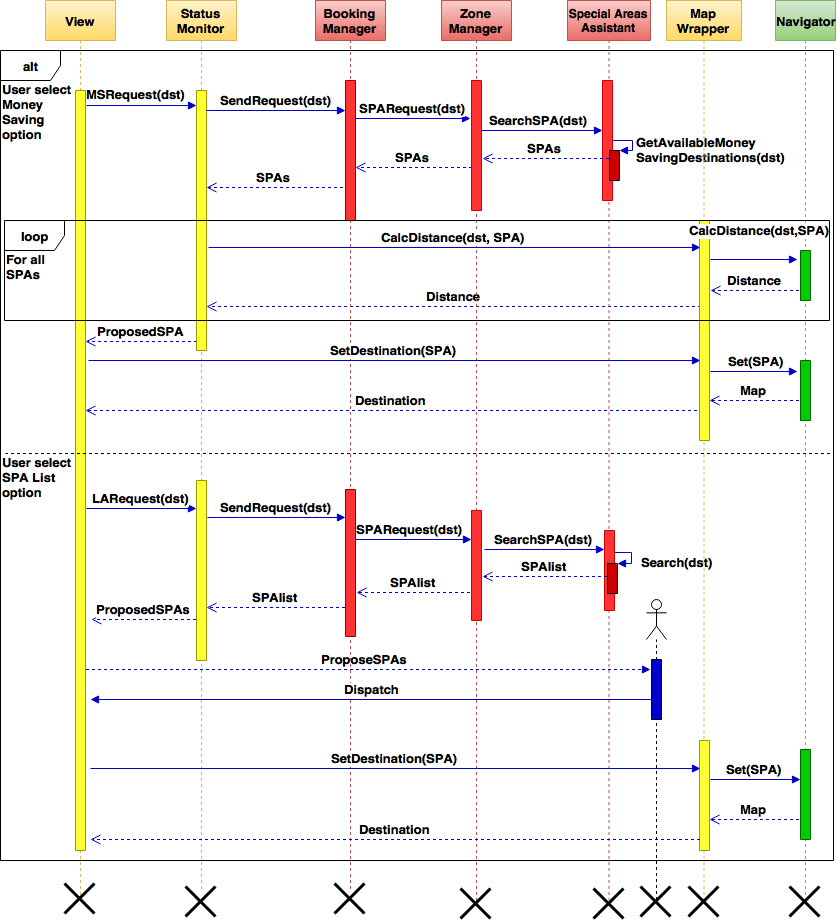
\includegraphics[scale=0.55]{{Figures/Sequence_Diagram/MS.png}}
\label{fig:UML Sequence Diagram: Money Saving and List Parking Area options}
\caption{Money Saving and List Parking Area options}
\end{figure}

\newpage

\subsection{Component interfaces}
In this section are defined the interfaces shown in the component view section. To make them easier to find they are listed in alphabetic order.
\begin{itemize}
    \item\textbf{IAccountable}\newline
    It is the interface to the Account Manager of the SBL through which it can handle requests about signing in, registration to the service and modification of account data.
    \item\textbf{IAccountingProvider}\newline
    It is the interface the Client API/Accounting component shows to client-side apps. Via this interface the Account component of client-side apps can access the functions needed to signing in, register a new user, modifying user data.
    \item\textbf{IBookable}\newline
    It is the interface to the SBL through which it can handle requests regarding positions of available Cars, their status, position of the reserved Car, unlocking of the reserved Car, positions of the Special Parking Areas close to the user provided destination, ride data, discounts and penalties applicability evaluation and any other active ride information.
    \item\textbf{IBookingProvider}\newline
    It is the interface the Client API/Booking component shows to client-side apps. Via this interface the apps can submit their request about Cars positions, Cars status, Car unlocking, Special Parking Areas locations, ride details.
    \item\textbf{IConnectable}\newline
    It is the interface that gives access to hardware sensor data of a vehicle. In particular about its location, the engine status, ignited or not, battery level and any other available sensor data.
    \item\textbf{IDataProvider}\newline
    It is the interface provided by the entity framework the PEJ Context relies on to get bidirectional access to data in form of object entities whenever one of the SBL components requests or store a piece of data.
    \item\textbf{IExplorable}\newline
    It is the interface in charge of providing the components which use it with the set of functions required to explore the map, such as zoom and scrolling.
    \item\textbf{IMailer}\newline
    It is the interface used to send to Mail Server the recipient email address and content that must be sent.
    \item\textbf{IManagableAccount}\newline
    It is the interface the Booking Handler relies on to get the data of the user who is making a reservation.
    \item\textbf{IMapProvider}\newline
    It is the interface the Map Wrapper uses to get the data on the map, but it provides other functions too; in particular the possibility to look for a specific address, and by doing so checking whether that address exists or not, and to get the distance between two provided locations.
    \item\textbf{INavigable}\newline
    It is the interface each View has to expose in order to support navigation and acceptance of input viewmodels.
    \item\textbf{IPaymentProvider}\newline
    It is the interface exposed by Payment Processor accepting payment requests and returning transaction outcome on completion.
    \item\textbf{IPaymentRequest}\newline
    It is the interface the Booking Handler uses to create a pending payment for a particular user. Via this interface the ride reference is passed to the Payment Processor in order to apply discounts or penalties before issuing the payment.
    \item\textbf{IQueryable}\newline
    It is the interface the Special Areas Assistant exposes to be queried about the positions of the Special Parking Areas, in particular via this interface the Zone Manager can answer to the Booking Handler requests about the list of the closest SPA to a provided location.
    \item\textbf{ITrackable}\newline
    It is the interface the Zone Manager uses to check the position and the other data of each vehicle. Furthermore it is via this interface that the Zone Manager can receive inform about engine ignition or shut down.
    \item\textbf{IViewable}\newline
    It is the interface that components with visual contents expose to the View component in order to provide the information and the data to be rendered.
    \item\textbf{IZoneService}\newline
    It is the interface the Zone Manager provides the Booking Handler with the set of functions required by the latter to accomplish its tasks, including getting vehicles location, asking for Car unlocking, asking for the closest set of SPA from a given location. Furthermore the Zone Manager uses this interface to notify the Booking Handler about vehicle status changes, such as location or engine ignition.
\end{itemize}


\subsection{Selected architectural styles and patterns}
The solution described in this document strongly embrace modern cloud-oriented philosophy. We believe the PowerEnJoy service has those key characteristics that made the choice of a cloud architecture to fit very nicely our customer needings.
As most significant ones we would like to underline:
\begin{itemize}
    \item The PowerEnJoy system will be developed from scratch, this allows the adoption of most convenient and future-proof architectural designs.
    \item PowerEnJoy is a start-up company, cloud Infrastructures as a Service are well-known to minimize initial deployment costs and risks of capital in case of business failure.
    \item Car sharing services, at the moment are experiencing a significant growth in terms of user adoption, therefore exists a concrete chance that the architecture would be heavy loaded even on service launch date which will probably require huge resources deployment that will take relatively long time to be completed with on-premise infrastructures.
\end{itemize}
\subsubsection{Cloud Design Patterns}
Designing cloud-ready software solutions has an immediate positive side-effect: each single taken design decision must always keep that elasticity and abstraction level the environment itself is characterized by. This practically turns out into helping solution architects to avoid many kinds of bad and harmful decisions that often come from technological concerns. The PowerEnJoy software platform this document describes follows most common recommended guidelines and best practices about roles subdivision across virtual compute units, message queuing and processing, data replication and caching. For more detailed description of those concepts you can refer to the MSDN library article you find in the External references section (§\ref{external_ref}) of this document.

\subsubsection{Architectural Design Patterns}
The whole PowerEnJoy software platform consists of a distributed, multi-tier architecture with a presentation layer split into a common front-end proxy and two different remote client-side apps, a middle tier that implements the PowerEnJoy business logic, a data tier which splits into multiple datasources and an IoT tier which includes both remote embedded devices and incoming telemetry data proxy. Each remote client-side app adopt an MVC style pattern, but its actual interpretation varies across different frameworks supported by the target OSs.

\subsubsection{Communication Design Patterns}
\label{com_patterns}
Given the distributed architectural layout, we had to keep particular attention designing each communication layer across various types of components. Where appropriate we have adopted a different approach always trying to leverage well-known design patterns in conjunction with open communication protocols that make much easier to integrate components based on heterogeneous technologies.\\

For interconnection of front-end and back-end roles a standard Enterprise Service Bus has been adopted. Being its queuing and dispatching mechanisms both REST-based and event-driven, it accommodates our necessity of distributing message processing workloads across multiple different worker instances.\\

Client-side apps are connected to front-end roles by typical REST-based Client-Server patterns but are also able to receive asynchronous messages from the server via standard push notification service which basically resemble a Publisher-Subscriber channel. All messages sent through REST channels are encoded in JSON format. The choice of JSON/REST protocol suite over XML/SOAP has been adopted to minimize network loads caused by unnecessary XML verbosity, and also to maximize compatibility with existing messaging services from major cloud providers.\\

The connection between Vehicle Embedded Platforms is built over open AMQP/1.0 protocol, which turns out to be the most efficient one that integrates all security and performance features that the communication to IoT devices is expected to have. Those AMQP messages are processed by an Event Hub, a kind of Service Bus specifically designed to collect event streams at high throughput, which makes it perfect for IoT telemetry and management scenarios.

\subsection{Other design decisions}
Following paragraphs refer to relevant design decisions not explicitly explained anywhere else in this document.\\

The SBL supports configurable timeout values for any event regarding a ride. This means no software upgrade is needed to change those values in case of requirements changes.\\

The SBL supports configurable discounts policies. This means that each required feature regarding discount applicability can be modified or updated in future without any software upgrade. Each discount policy is defined by a set of conditions to be satisfied at a specific point of a booking (on Car unlocking, on engine turn-off, on Car locking) and parameters that allow to modify the charged fare (percentage discount ratio, absolute discount amount).\\

As said in previous chapters, each zone served by PowerEnJoy can override any global setting from the shared configuration datasource.\\
    
The client-side apps are expected to evolve much more frequently with respect to other service components. Therefore sounds reasonable not to define further the MVC pattern variant technicalities, taking advantage of any platform specific framework which best integrates with the target at the time of development. These components are designed such that the development of a brand-new version based on a completely different MVC framework should complete in short time and without generating issues to be addressed into other components of the solution, in the event of new target OSs release/update.
\newpage
\section{Algorithm Design}


\subsection{Getting money saving destination}

\subsubsection{Part 1}

The first algorithm runs in the Special Areas Assistant component and it takes care of looking for the available Special Parking Areas located inside a certain range from the specified destination.

\begin{itemize}
    \item The \textit{isFull} method returns true if the Special Parking Area is full and no further vehicle can be parked there and plugged to the power grid.
    \item The \textit{getRange} method returns the value of the range of the provided zone.\newline
    This way the algorithm can be adapt to zones with different conformations just by changing the value of the range.
    \item The \textit{calcAirDistance} method returns the air distance from the provided position to the the known position of the provided Special Parking Area. The air distance is used in order to keep low the level of the required computational power.
\end{itemize}

\begin{algorithm}
\caption{}\label{euclid}
\begin{algorithmic}[1]
\Function{getAvailableMoneySavingDestinations}{\textit{DestPosition}}
\State \textit{var MSDestinations}[] = \textit{empty}
\State \textit{var SpecialParkAreas}[] = \textit{PEJContex}.\textit{getSPAreas}(\textit{DestPosition}.\textit{getZone})
\For {(\textit{int i}=0; \textit{i}<\textit{SpecialParkAreas}[].\textit{count}; \textit{i}++)}
\If {\textit{not}(\textit{SpecialParkAreas}[\textit{i}].\textit{isFull}) \textit{and}
\State (\textit{PEJContex.\textit{getRange}(\textit{DestPosition}.\textit{getZone})}>\State\textit{calcAirDistance}(\textit{DestPosition},\textit{ SpecialParkAreas}[\textit{i}]))}
\State \textit{MSDestinations}[].\textit{append}(\textit{SpecialParkAreas}[\textit{i}])
\EndIf
\EndFor
\State \Return \textit{MSDestinations}[]
\EndFunction
\State \textbf{end function}
\end{algorithmic}
\end{algorithm}


%\newpage
\subsubsection{Part 2}

The second algorithm runs in the Status Monitor \textbf{MUST BE CONSISTENT WITH THE SEQUENCE DIAG} component and it uses the list of feasible Special Parking Areas returned by the previous algorithm to establish which one is actually the closest to the destination.

\begin{itemize}
    \item The \textit{calcDistance} method returns the street distance from the provided position to the the known position of the provided Special Parking Area contained in \textit{MSDestinations}. This real world distance is provided relying on the Navigator that can compute the actual distance between two provided positions.
\end{itemize}

\begin{algorithm}
\caption{}\label{euclid}
\begin{algorithmic}[1]
\Function{getMoneySavingDestination}{\textit{MSDestinations}[]}
\State \textit{var Distance =99999}
\If{\textit{MSDestinations}[]==\textit{empty}}
\State\Return \textit{errorMsgNoMoneySavingDestinationFound}
\EndIf
\For{\textit{int i}=0; \textit{i}<\textit{MSDestinations}.\textit{count}[]; \textit{i}++}
\If {(\textit{Distance}>\textit{calcDistance}(\textit{DestPosition}, \textit{MSDestinations}[\textit{i}]))}
\State \textit{Distance} = \textit{calcDistance}(\textit{DestPosition}, \textit{MSDestinations}[\textit{i}])
\State \textit{MSDestination} = \textit{MSDestinations}[\textit{i}]
\EndIf
\EndFor
\State\Return \textit{MSDestination}
\EndFunction
\State \textbf{end function}
\end{algorithmic}
\end{algorithm}

\newpage


\subsection{Total Ride Fare}
This algorithm runs in the Payment Processor component and it takes care of applying any discount or penalty the user is eligible for at the end of the ride. In case the user has never started the ride, after the reservation expiration, this algorithm applies the penalty fee. Furthermore, it checks whether the user has any pending payment in order to add it to the total ride fare.

\begin{itemize}
    \item The \textit{getTotalBaseFare} method returns the Total Base Fare value which depends only on the amount of time of the Ride.
    \item The \textit{hasStarted} method returns true if the user has ignited the engine of the Car at least one; otherwise returns false.
    \item The \textit{getDiscounts} method is provided via PEJ Context, given a zone it returns the discounts and the penalties that can be applied in that particular zone.\newline
    This way this algorithm can adapt to new discounts or penalties, or to removal of one of them, without needing of any modification.
    \item The \textit{isApplicable} method returns true if that particular discount can be applied to that particular ride.
    \item The \textit{applyDiscount} method compute the new value of the Total Ride Fare after the applicatin of the discount or penalty.
    \item The \textit{getExpirationFee} method returns the amount of fee the user is charged with in case of expired reservation.
    \item The \textit{hasPendingPayment} method return true if there is at least one payment for that particular user that has not completed successfully and still need to be collected.
     \item The \textit{getPendingPaymentValue} method return the value of the money the user still owe the company from previous rides.
\end{itemize}

\begin{algorithm}
\caption{}\label{euclid}
\begin{algorithmic}[1]
\Function{caculateTotalRideFare}{\textit{Ride}}
\State \textit{var TotalRideFare} = \textit{Ride}.\textit{getTotalBaseFare}
\If {\textit{Ride}.\textit{hasStarted}}
\For{(\textit{Discount} \textbf{in} \textit{PEJContex}.\textit{getDiscounts}(\textit{Ride}.\textit{getZone}))}
\If{\textit{Ride}.\textit{isApplicable}(\textit{Discount})}
\State \textit{TotalRideFare}=\textit{TotalRideFare}.\textit{applyDiscount}(\textit{Discount})
\EndIf
\EndFor
\Else
\State \textit{TotalRideFare} = \textit{PEJContex}.\textit{getExpirationFee}(\textit{Ride}.\textit{getZone})
\EndIf
\If {\textit{Ride}.\textit{getUser}.\textit{hasPendingPayment}}
\State \textit{TotalRideFare}+=\textit{Ride}.\textit{getUser}.\textit{getPendingPaymentValue}
\EndIf
\State \Return \textit{TotalRideFare}
\EndFunction
\State \textbf{end function}
\end{algorithmic}
\end{algorithm}

\leavevmode\thispagestyle{empty}\newpage
\newpage
\section{User Interface Design}
Fully explained mockups of the user interface can be found in the RASD document.\newline In this section are presented the UX diagrams of the user experience of both mobile app and Car app.

\begin{figure} [p!]
\centering
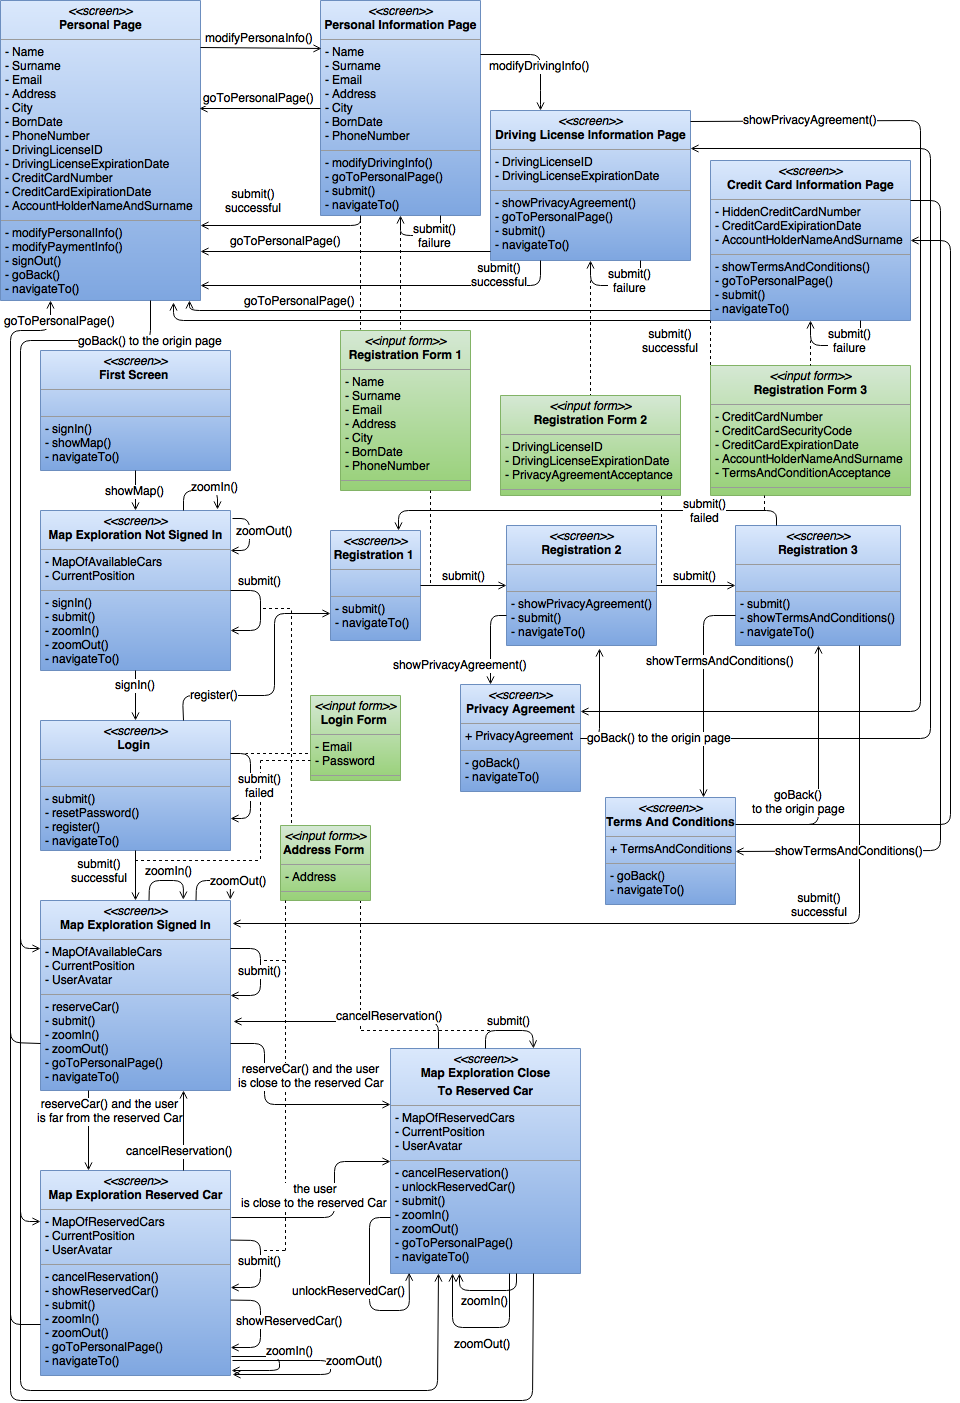
\includegraphics[scale=0.4]{{Figures/UX_Diagram/UXMobileApp.png}}
\caption{Mobile app}
\label{fig:UXMobileApp}
For better readability, two larger images of the same diagram have been put after this full complete one. 
\end{figure}

\begin{landscape}
\begin{figure} [p!]
\centering
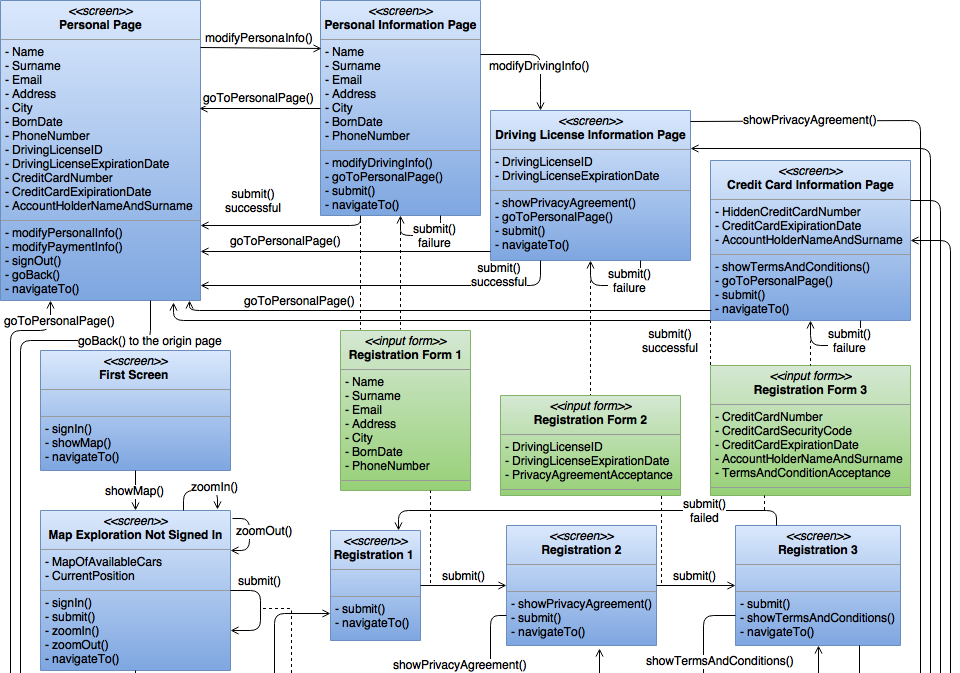
\includegraphics[scale=0.6]{{Figures/UX_Diagram/UXMobileApp-part1.png}}
\caption{Mobile app - part 1}
\label{fig:UXMobileApp-part1}
\end{figure}

\begin{figure} [p!]
\centering
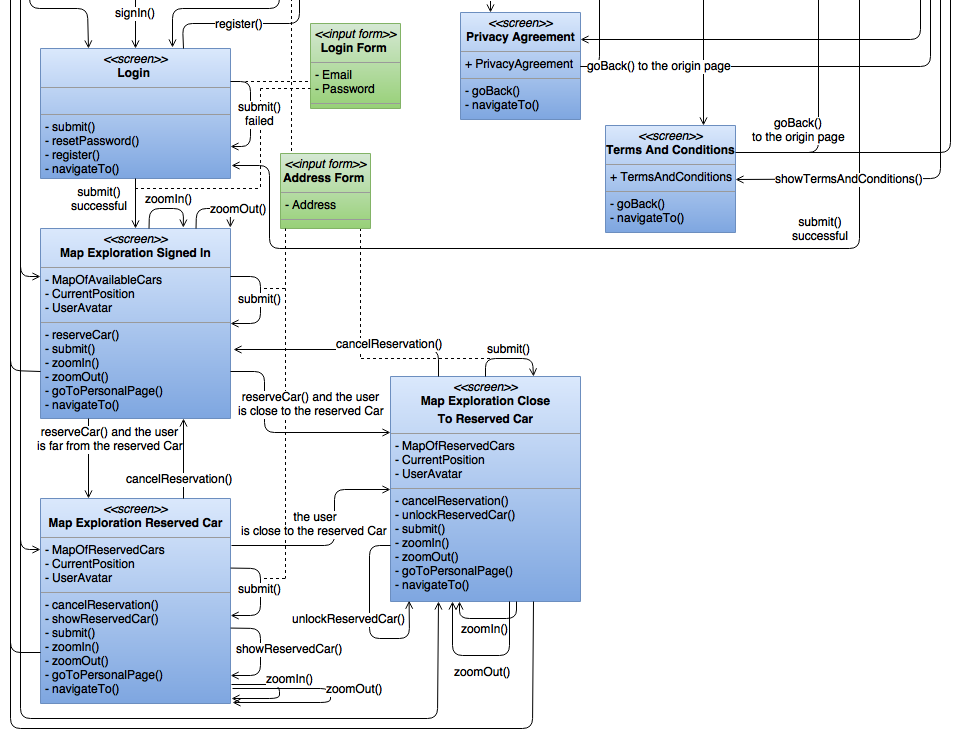
\includegraphics[scale=0.6]{{Figures/UX_Diagram/UXMobileApp-part2.png}}
\caption{Mobile app - part 2}
\label{fig:UXMobileApp-part2}
\end{figure}
\end{landscape}

\begin{figure} [h!]
\centering
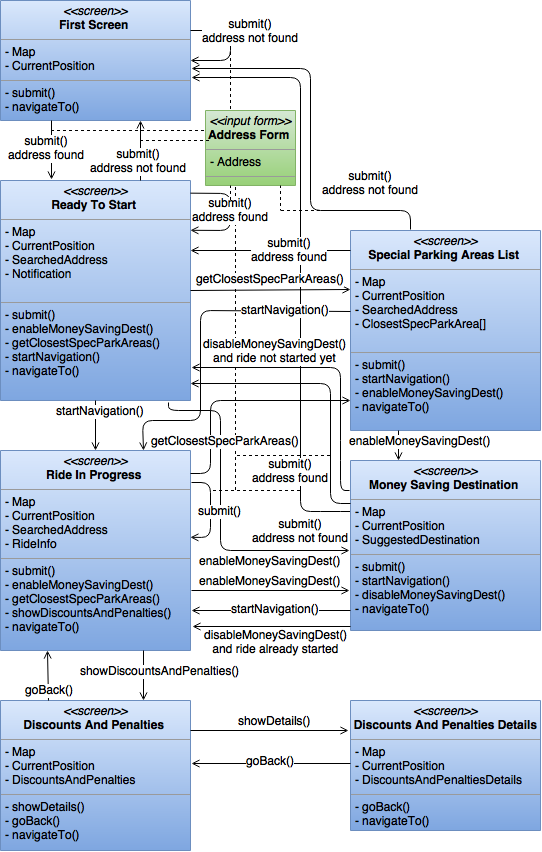
\includegraphics[scale=0.6]{{Figures/UX_Diagram/UXCarApp.png}}
\caption{Car app}
\label{fig:UXCarApp.png}
\end{figure}
\newpage
\section{Requirements Traceability}

\subsection {Goal 1} Allow any kind of user to view the map of the available nearby Cars.
\begin{itemize}
 \item |R1| Users must have access to a map indicating the user current location.
    \newline - 2.2.2 Map Explorer component.
    \newline - 4 User Interface Design Figure 4.
 \item |R2| Users must be able to pan and scroll a map in any direction.
    \newline - 2.2.2 Map Wrapper component.
    \newline - 4 User Interface Design Figure 4.
 \item |R3| Every available Car must be shown on a map.
     \newline - 2.2.2 Map Explorer component.
     \newline - 4 User Interface Design Figure 4.
 \item |R4| Users shall have an input for inserting an address in which center the map.
    \newline - 2.2.2 View component.
    \newline - 4 User Interface Design Figure 4.
 \item |R5| Users shall have an input to center the map view on their position.
    \newline - 2.2.2 View component.
    \newline - 4 User Interface Design Figure 4.
\end{itemize}

\subsection {Goal 2} Allow Visitor user to register to the service.
\begin{itemize}
 \item |R6| Let a Visitor user start the registration wizard while he's still not logged in.
    \newline - 2.2.2 View \& Account components.
    \newline - 4 User Interface Design Figure 4.
 \item |R7| The registration form must contain input fields for user identity, email, contact
info, driving license number and expiration, privacy agreement confirmation,
credit card number and expiration, billing identity.
    \newline - 2.2.2 View \& Account components.
    \newline - 4 User Interface Design Figure 4.
 \item |R8| The chosen email address must not be already used by another PowerUser.
    \newline - 2.2.1 Account component.
    \newline - 4 User Interface Design Figure 4.
 \item |R9| The credit card must be verified not to be blocked or expired upon registration.
    \newline - 2.2.1 Account component.
    \newline - 4 User Interface Design Figure 4.
 \item |R10| The user must receive a system generated password to the registered email
address.    
    \newline - 2.2.1 Account component.
    \newline - 4 User Interface Design Figure 4.
\end{itemize}

\subsection {Goal 3} Allow Visitor user to log-in and out as a PowerUser.
\begin{itemize}
 \item |R11| A Visitor user must always see an input to access log-in form as long as he's
still not logged in.
    \newline - 2.2.2 View \& Account components.
    \newline - 4 User Interface Design Figure 4.
 \item |R12| An input to perform log-out must always be available to the PowerUser if he's
currently logged in.
    \newline - 2.2.2 View \& Account components.
    \newline - 4 User Interface Design Figure 4.
\end{itemize}

\subsection {Goal 4} Allow PowerUser to check the status of the Car.
\begin{itemize}
 \item |R13| For each available Car the PowerUser must be able to view its remaining
battery charge.
    \newline - 2.2.2 Map Explorer component.
    \newline - 4 User Interface Design Figure 4.
 \item |R14| For each available Car the PowerUser must be able to view its current position.
    \newline - 2.2.2 Map Explorer component.
    \newline - 4 User Interface Design Figure 4.
\end{itemize}

\subsection {Goal 5} Allow PowerUser to reserve a Car.
\begin{itemize}
 \item |R15| The PowerUser must have the ability to start the reservation wizard for all
and only available Cars.
    \newline - 2.2.2 Map Explorer component.
    \newline - 4 User Interface Design Figure 4.
 \item |R16| The PowerUser must see a reminder about unfulfilled reservation penalty before
confirmation.
    \newline - 2.2.2 Map Explorer component.
    \newline - 4 User Interface Design Figure 4.
 \item |R17| Show an input to allow the PowerUser to confirm and finalize the reservation.
    \newline - 2.2.2 Map Explorer component.
    \newline - 4 User Interface Design Figure 4.
 \item |R18| The system shall prevent the PowerUser to reserve more than a Car from the same geographical region at a time.
    \newline - 2.2.1 Booking Handler component.
\end{itemize}

\subsection {Goal 6} Allow PowerUser to cancel a reservation.
\begin{itemize}
 \item |R19| If a reservation exists for the PowerUser, show him an input to request cancellation.
    \newline - 2.2.2 Reserved Car Viewer component.
    \newline - 4 User Interface Design Figure 4.
 \item |R20| The system shall prompt the PowerUser for cancellation confirmation.
    \newline - 2.2.1 Booking Handler component.
    \newline - 4 User Interface Design Figure 4.
 \item |R21| A reservation must be automatically cancelled by the system after 1 hour from
its creation.
    \newline - 2.2.1 Booking Handler component.
 \item |R22| If a reservation is cancelled because of timeout, notify the PowerUser about
that occurrence.
    \newline - 2.2.1 Booking Handler component.
\end{itemize}

\subsection {Goal 7} Allow PowerUser to check the position of the reserved car.
\begin{itemize}
 \item |R23| As long as a reservation exists for the PowerUser he must always be able to
get the position of the reserved Car on the map.
    \newline - 2.2.2 Reserved Car Viewer component.
    \newline - 4 User Interface Design Figure 4.
\end{itemize}

\subsection {Goal 8} Allow PowerUser to unlock and enter the Car when inside the specific range.
\begin{itemize}
 \item |R24| The system must be able to remotely unlock the Car.
    \newline - 2.4 Runtime View Figure 1.
    \newline - 2.2.1 Booking Handler component.
 \item |R25| The system must be able to compute the distance between the user location
and his reserved Car.
    \newline - 2.4 Runtime View Figure 1.
    \newline - 2.2.1 Booking Handler component.
 \item |R26| The PowerUser must have an input allowing him to send an unlock request.
    \newline - 2.4 Runtime View Figure 1.
    \newline - 2.2.2 Reserved Car Viewer component.
    \newline - 4 User Interface Design Figure 4.
 \item |R27| The system must accept the unlock request issued by the PowerUser if and only if the PowerUser is in the unlock allowance area.
    \newline - 2.4 Runtime View Figure 1.
    \newline - 2.2.1 Booking Handler component.
 \item |R28| If the unlock request is accepted, the PowerUser must be able to enter the Car.
\newline - 2.4 Runtime View Figure 1
\end{itemize}

\subsection {Goal 9} Allow PowerUser to get driving directions to his destination.
\begin{itemize} 
 \item |R29| The user must be allowed to select a custom destination and start navigating
to that location.
    \newline - 2.4 Runtime View Figure 2.
    \newline - 2.2.3 Map Wrapper component.
\end{itemize}

\subsection {Goal 10} Bill the PowerUser for the amount of time spent riding a Car.
\begin{itemize}
 \item |R30| Start counting the billing time from the first engine ignition.
    \newline - 2.2.2 Booking Handler component.
 \item |R31| Stop the billing time counter exactly 1 second after the Car locking.
    \newline - 2.2.2 Booking Handler component.
\end{itemize}

\subsection {Goal 11} Allow PowerUser to see a list of the closest Special Parking Areas to his destination.
\begin{itemize}
 \item |R32| The system must be capable of providing a list of Special Parking Areas sorted
by distance from an input location.
     \newline - 2.4 Runtime View Figure 2 \& Figure 3.
     \newline - 4 User Interface Design Figure 7.

 \item |R33| PowerUser must be allowed anytime during the navigation to input a custom location and be acknowledged about all nearest Special Parking Areas from the selected location.
    \newline - 2.4 Runtime View Figure 2 \& Figure 3.
    \newline - 2.2.3 Map Wrapper \& View components.
    \newline - 4 User Interface Design Figure 7.
\end{itemize}

\subsection {Goal 12} Allow PowerUser to keep track of the Current Fare.
\begin{itemize}
 \item |R34| Show on the Car screen a live updated counter indicating the Current Fare amount that the user would actually pay if the ride ended in that same moment,as long as the ride is being charged.
    \newline - 2.2.3 Status Monitor component.
    \newline - 4 User Interface Design Figure 7.
\end{itemize}

\subsection {Goal 13} Allow PowerUser to check whether he can be eligible for any discount or penalty.
\begin{itemize}
 \item |R35| Provide through Car screen an input to access an overview of all discounts
and penalties.
    \newline - 2.2.3 Status Monitor component.
    \newline - 4 User Interface Design Figure 7.
 \item |R36| For each shown discount or penalty allow the PowerUser to get a brief informal description of corresponding criteria.
    \newline - 2.2.3 Status Monitor component.
    \newline - 4 User Interface Design Figure 7.
 \item |R37| For each shown discount or penalty allow the PowerUser to know if the current ride satisfies all needed criteria at the moment.
    \newline - 2.2.3 Status Monitor component.
    \newline - 4 User Interface Design Figure 7.
\end{itemize}

\subsection {Goal 14} Allow PowerUser to get a money saving alternative destination.
\begin{itemize}
 \item |R38| Show the PowerUser the option to get a money saving destination alternative after entering desired destination address.
    \newline - 2.4 Runtime View Figure 2 \& Figure 3.
    \newline - 3.1.1 Algorithm design Algorithm 1 \& 2.   
    \newline - 4 User Interface Design Figure 7.
 \item |R39| Always show to PowerUser an input to get money saving proposal even if there already exists a selected destination.
    \newline - 2.4 Runtime View Figure 2 \& Figure 3.
    \newline - 4 User Interface Design Figure 7.
 \item |R40| The destination proposal must correspond to the nearest (w.r.t. PowerUser selected destination) Special Parking Area where there are less than N\# Cars attached to the power source.
    \newline - 2.4 Runtime View Figure 2 \& Figure 3.
    \newline - 3.1.1 Algorithm design Algorithm 1 \& 2. 
 \item |R41| If the PowerUser accepts the money saving destination proposal, the current selected destination must be updated accordingly.
    \newline - 2.4 Runtime View Figure 2 \& Figure 3.
    \newline - 4 User Interface Design Figure 7.
\end{itemize}

\subsection {Goal 15} Allow the system to lock the Car in a Safe Parking Area at the end of the ride.
\begin{itemize}
 \item |R42| The system must lock the Car if its position belong to the set of Safe Parking
Areas, engine is stopped, all doors are closed and S\# seconds passed from the
last door closure.
    \newline - 2.2.1 Booking Manager component.
\end{itemize}

\subsection {Goal 16} Allow the system to apply penalty or discount according to the given criteria.
\begin{itemize}
 \item |R43| The system shall apply a discount of 10\% on the last ride Total Base Fare if the number of passengers at the end of the ride is greater or equal to the number of passengers at the start of the ride and the number of passengers at the start of the ride was at least 3, driver included.
    \newline - 2.2.1 Booking Manager component.   
 \item |R44| The system shall apply a discount of 20\% on the last ride Total Base Fare if the remaining battery power at the end of the ride is greater or equal then 50\%.
    \newline - 2.2.1 Booking Manager component.
 \item |R45| The system shall apply a discount of 30\% on the last ride Total Base Fare if
the Car position at the end of the ride is within a Special Parking Areas and
the power socket is detected as connected two minutes from the Car locking.
    \newline - 2.2.1 Booking Manager component.
 \item |R46| The system shall apply a penalty of 30\% on the last ride Total Base Fare if the position of the Car at the time of locking is more than 3km far from the nearest power grid station, or the remaining battery power is less than 20\% and the Car is not detected as attached to power grid within two minutes from locking.
    \newline - 2.2.1 Booking Manager component.
\end{itemize}

\subsection {Goal 17} Let the system bill the PowerUser for the Total Ride Fare and issue a payment
request for that amount at the end of the ride.
\begin{itemize}
 \item |R47| The system must charge the PowerUser the Total Ride Fare after two minutes
and an half from the Car locking.
    \newline - 2.2.1 Booking Manager component.
 \item |R48| The system must issue the payment request to the Payment Processor Provider.
    \newline - 2.2.1 Payment Processor component.
 \item |R49| The system must bill the PowerUser a penalty of 1e as soon as a reservation
he made expires by timeout.
    \newline - 2.2.1 Booking Manager component.
 \item |R50| The PowerUser shall be notified of any money charge by email.
    \newline - 2.2.1 Account Manager component.
 \item |R51| The PowerUser shall be notified of the payment transaction result.
    \newline - 2.2.1 Account Manager component.
\end{itemize}
\newpage
\section{Effort Spent}
\begin{tabular}{| p{5cm} | p{5cm} |}
\hline
Teamwork & $\sim$?h\\
\hline
Piccirillo Luca & $\sim$?h\\
\hline
Zampogna Gian Luca & $\sim$?h\\
\hline
Zini Edoardo & $\sim$?h\\
\hline
\end{tabular}

\newpage
\section{References}

%if you remove this section be sure to update the counter in the text of the paragraph 1.5 Document Structure!!!!!!!!!

\subsection{Reference documents}
See section 1.4.



\subsection{Document revisions history}
\begin{tabular}{| l | l | p{10cm} |}
\hline
\textbf{Version} & \textbf{Date} & \textbf{Changes}\\
\hline
1.0-RC1 & 11/12/2016 & First deadline release.\\
\hline
\end{tabular} 

\end{document}